%!TEX root = ../thesis.tex
%*******************************************************************************
%*********************************** First Chapter *****************************
%*******************************************************************************

\chapter{The Future of High Energy Physics }  %Title of the First Chapter

\ifpdf
    \graphicspath{{Introduction/Figs/Raster/}{Introduction/Figs/PDF/}{Introduction/Figs/}}
\else
    \graphicspath{{Introduction/Figs/Vector/}{Introduction/Figs/}}
\fi


%********************************** %First Section  **************************************

\begin{wrapfigure}{R}{0.5\textwidth}
\centering    
    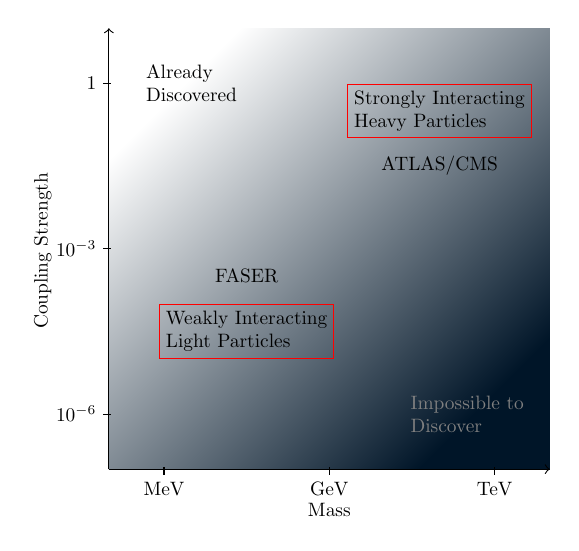
\begin{tikzpicture}[only marks,scale=0.7, every node/.style={scale=0.7}]
        \definecolor{deepblue} {HTML}{001528}
        \shade[top color=white,bottom color=deepblue, shading angle = 45] (0,0) rectangle (8,8);
        \node[draw=red, align=left] (wimp) at (2.5,2.5) {Weakly Interacting \\ Light Particles};
        \node[above of=wimp] {FASER};
        \node[align=left] at (1.5,7) {Already \\ Discovered};
        \node[draw=red, align=left] (sihp) at (6,6.5) {Strongly Interacting \\ Heavy Particles};
        \node[below of=sihp] {ATLAS/CMS};
        \node[align=left, text=gray] at (6.5,1) {Impossible to \\ Discover};
        \draw[->] (0,0) -- coordinate (x axis mid) (8,0);
        \draw[->] (0,0) -- coordinate (y axis mid) (0,8);
        \foreach \x/\xtext in {1/MeV,4/GeV,7/TeV}
            \draw (\x cm,1pt) -- (\x cm,-3pt) node[anchor=north] {\xtext};
        \foreach \y/\ytext in {1/10^{-6},4/10^{-3},7/1}
            \draw (1pt,\y cm) -- (-3pt,\y cm) node[anchor=east] {$\ytext$};
        \node[below=0.5cm] at (x axis mid) {Mass};
        \node[left=1.2cm,rotate=90,xshift=1.5cm] at (y axis mid) {Coupling Strength};
    \end{tikzpicture}    
\caption[Diagram coupling strenght vs Mass]{ATLAS and CMS focus on large transverse momentum ($p_{T}$) signatures that emerge in the roughly isotropic decay of such particles. There is a complementary class of viable new particles that are much lighter, with mass in the MeV to GeV range, much more weakly coupled to the SM.}
\label{fig:CouplingStrength_Mass}
\end{wrapfigure}

\section{Introduction} %Section - 1.1 

The Large Hadron Collider (LHC) is one of the wonders of the modern world - the largest and highest-energy particle collider designed to explore the laws governing the interactions and forces among the fundamental particles, the structure of space and time and the correlation between quantum mechanics and general relativity. It has achieved to study in great detail the Standard Model as well as discover the Higgs boson, the particle that gives mass to all other particles. Nevertheless, many fundamental questions remain open in physics such as the apparent violation of symmetry between matter and antimatter, the Hierarchy problem between the four fundamental forces and the Grand Unification Theories, to name a few.
After the discovery of the Higgs boson, no physics beyond the standard model (SM) has been found at the LHC, which motivates the exploration of unprobed regions such as the search for light and weakly coupled long-lived particles.

ForwArd Search ExpeRiment (FASER) is a small and inexpensive detector installed in the far forward region of proton-proton ($pp$) collisions that will collect data during Run 3 and probe new regions of the parameter space for new particles with masses in the 10 MeV to GeV range.
FASER requires no beam modifications and only requests luminosity  information. Further into the future, a larger
 FASER 2 will extend the sensitivity to even larger masses but will require significant civil engineering.

\section{How does FASER fit in the context of ATLAS and CMS}  %Section - 1.3 
\label{section1.3}

\begin{wrapfigure}[20]{L}{0.40\textwidth}
  \centering
    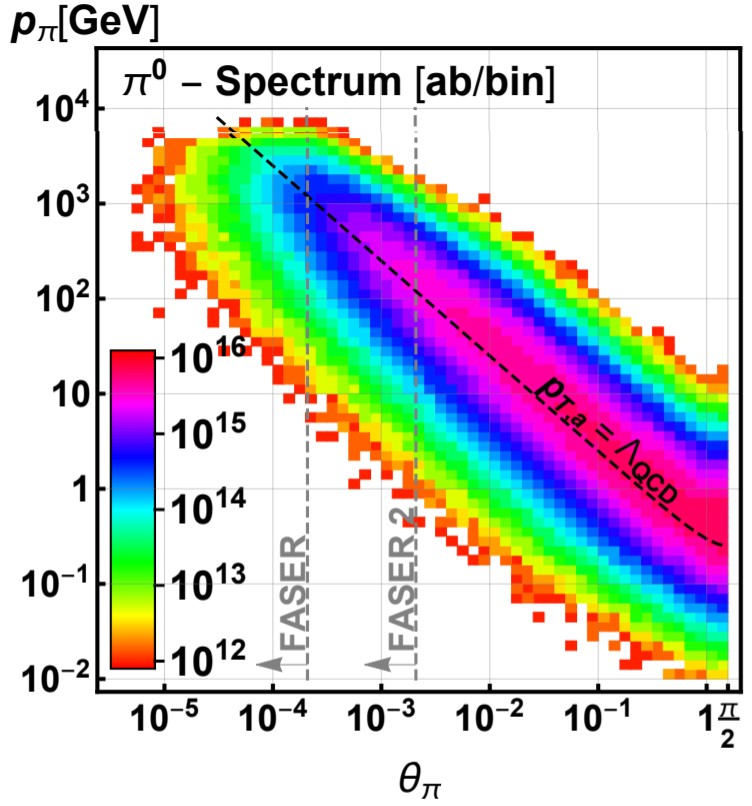
\includegraphics[width=0.38\textwidth]{Introduction/Figs/Raster/momentumVSangle.jpg} 
    \caption[Momentum vs angle]{Differential $\pi^{0}$ production rate in the ($\theta$, p) plane, where $\theta$ and p are the meson’s angle with respect to the beam axis and momentum, respectively. The angular acceptances for FASER and FASER 2 are indicated by the vertical gray dashed lines \cite{faser_collaboration_fasers_2019}.}
    \label{fig:momentumVSangle}
\end{wrapfigure}

The four main LHC experiments (ATLAS, CMS, ALICE, LHCb) that search for TeV-scale particles with high transverse momentum ($p_{T}$) may be misguided in the search for new particles. An area that isn't covered by these experiments, is the search for light particles with masses in the MeV to GeV range with low $p_{T}$. These new particles, that might be extremely weakly-coupled, may travel hundreds of meters without interacting with any material before decaying into known SM particles. During their travel, they would not be bent by magnets. Instead, they will continue along a straight line and only their decay products can be spotted by the FASER experiment. These hypothetical new particles would be long lived (LLP) and very collimated with the beam (of the order of the milliradian) allowing a small and inexpensive detector. For example, new particles that are produced in pion or B-meson decays are typically produced within angles \[ \theta\sim\frac{\Lambda_{QCD}}{E}\sim\frac{m_{pion}}{E} \] of the beam collision axis, where E is the energy of the particle and $\Lambda_{QCD}$ is the scale of the pion mass. This implies that around 500 meters after the interaction point the downstream particle spread is 10 to 100 cm \cite{faser_collaboration_letter_2018}. FASER will search for light and extremely weakly interacting particles in the far forward region of the LHC where a large number of mesons ($10^{16}$ pions per year) is expected, as shown on Fig. \ref{fig:momentumVSangle}. This large production rate, needed if these particles are weakly coupled, might allow to find dark photons ($A'$) - a product of the decay of pions - that are otherwise swamped in background at higher $\theta$, within the ATLAS detector. The mesons would decay in ATLAS ($\pi^{0}\rightarrow A'\gamma$) and the $A'$ would travel and decay in FASER, situated 480 m along the line-of-sight of the proton collisions in front of the ATLAS interaction point at the LHC. It has the prospect of discovering new particles such as dark photons, dark Higgs bosons, heavy neutral leptons and axion-like particles - produced in LHC collisions via high energy
photons interacting with material in the LHC neutral particle absorber
(TAN). FASER is part of the CERN's Physics Beyond Colliders study group which is an exploratory study aimed at exploiting the full scientific potential of CERN's accelerator complex and its scientific infrastructure through projects complementary to the existing LHC, HL-LHC and other possible future colliders. The cost of the
experiment is less than 1 MCHF and funding has been secured from the Simons and Heising-Simons foundations.

\subsection{Beyond the Standard Model}

\begin{wrapfigure}{R}{0.25\textwidth}
  \centering
    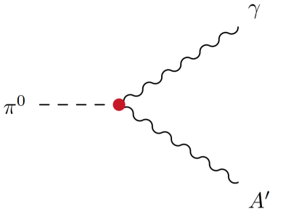
\includegraphics[width=0.24\textwidth]{DarkPhoton.png} 
    \caption[Neutral Pion Decay]{Neutral pion to dark photon decay.}
    \label{fig:Dark Photon}
\end{wrapfigure}

The FASER collaboration hopes to discover new particles through this experiment. An example for such a new particles is the dark photon, Fig.\ref{fig:Dark Photon}. Dark photons are hypothetical hidden sector (a collection of yet unobserved quantum fields) particles. Interaction between hidden sector and SM are weak, indirect and would be mediated via gravity or new particles. Dark photons are proposed as a force carrier, similar to the photon in the SM with a new abelian U(1) gauge symmetry. This new spin-1 gauge boson could couple very weakly to electrically charged particles through kinetic mixing with the normal photon \cite{noauthor_dark_2019}.
They could be produced in meson decays, where we see that the branching ratio (B) of the neutral pion to $A'$ and a photon is the same as the branching ratio for $\pi^0 \rightarrow \gamma\gamma$ but modified by the mass of  the $A'$:
\[
B(\pi^0 \rightarrow A'\gamma)=2\epsilon^2\left( 1-\frac{m^2_{A'}}{m^2_{\pi^0}} \right)^3B(\pi^0 \rightarrow \gamma\gamma)
\]

\begin{wrapfigure}{L}{0.28\textwidth}
  \centering
    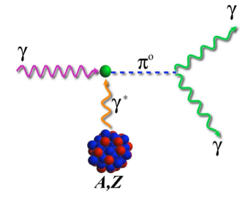
\includegraphics[width=0.26\textwidth]{Primakoff.png}
    \caption[Primakoff Effect]{The Primakoff effect is the resonant production of neutral pseudoscalar mesons by high-energy photons interacting with an atomic nucleus \cite{kang_standard_1978}.}
    \label{fig:Primakoff}
\end{wrapfigure}

Another type of new physics could be the discovery of axion-like-particles (ALPs). ALPs are hypothetical particles supposed stable, neutral and of very low mass (1 meV-$\mu$eV). They are a solution by Peccei-Quinn to the problem of CP violation in QCD.
There exists a possibility of using the LHC as a beam-dump experiment. Very high energy photons produced in the IP could interact with material in the Neutral Beam Absorbers (TAN, see Fig. \ref{fig:infrastructure}) and produce ALPs (~TeV energy) via Primakoff effect that could decay in FASER.



%********************************** % Nomenclature  *************************************
\nomenclature[z-PBC]{PBC}{Physics Beyond Colliders}
\nomenclature[z-CERN]{CERN}{Conseil Européen pour la Recherche Nucléaire}
\nomenclature[z-LHC]{LHC}{Large Hadron Collider}
\nomenclature[z-HL]{HL}{High Luminosity}
\nomenclature[z-ATLAS]{ATLAS}{A Toroidal LHC ApparatuS}
\nomenclature[z-eV]{eV}{Electronvolt}
\nomenclature[a-pt]{$p_{T}$}{Transverse Momentum}
\nomenclature[a-pp]{$pp$}{Proton-proton}
\nomenclature[z-SM]{SM}{Standard Model}
\nomenclature[z-IP]{IP}{Interaction Point}
\nomenclature[z-ALP]{ALP}{Axion like particles}
\nomenclature[z-CMS]{CMS}{Comact Muon Solenoid}